\documentclass[12pt,a4paper]{article}
\usepackage[utf8]{inputenc}
\usepackage{times}
\usepackage{hyperref}
\usepackage{graphicx}
\usepackage{listings}
\usepackage[english]{babel}

\begin{document}
\begin{titlepage}
	\centering
	
\includegraphics[width=0.66\textwidth]{src/title_logo.png}\par\vspace{1cm}
	{\scshape\LARGE Polytech Montpellier\par}
	\vspace{1cm}
	{\scshape\Large WOA Project\par}
	\vspace{1.5cm}
	{\huge\bfseries MenexaTech\par}
	\vspace{2cm}
	{\Large\itshape Yannick Mayeur\par}
	\vfill
	supervised by\par
	Arnaud \textsc{Castelltort}\par
	and\par
	Anne \textsc{Laurent}

	\vfill

% Bottom of the page
	{\large \today\par}
\end{titlepage}

\tableofcontents
\break


\section{Introduction}

When preparing for an exam it is good to know, what the exam may look like, and
what the teacher expects the students to know. Sadly this is not always
possible, because the previous exams of a given course are not always made
available by the teachers or the students that took it. At Polytech in IG a
google drive folder with some old exams exists. This is already very good, but
what would be even better is a place where students could get all of these
resources and also have a place to discuss them. That is how the idea for
MenexaTech was born. MenexaTech is a web application allowing students to
learn in a more effective way. By enabling  them to share previous exams and
offering them a place for discussion.


\section{Presentation of MenexaTech}

MenexaTech allows users, most of which are probably students, to follow or not
a certain number of courses. These courses all have a certain number of old
exams the user can download and each of them has a little forum where users
can discuss there answers.

Some Users are admins, to be an admin you will have to be a class
representative. Admins have the power to create and edit courses, as well as
old exams.


\section{Instructions}



\section{Technologies}

\subsection{Ruby on Rails}
To develop my web application I choose to use the Rails framework.
Rails is running on the Ruby programming language. Rails being a mature
framework, countless resources to help get started are available. The framework
once taken in hand helps build REST compliant applications more easily. One
of its design paradigms is "convention over configurations". This appealed to
me a lot because configuring something you do not entirely understand is always very
hard, and takes a lot of time. Moreover, Rails is easily testable with unit and
integration tests. This is very good to be sure no new functionality breaks
another part of the application.

\begin{figure}[h]
   \centering
   
\includegraphics[scale=0.1]{src/rails_logo.png}
   \caption{\label{fig:rlogo} Ruby on Rails logo}
\end{figure}


\subsection{Heroku}
To deploy my web application I used Heroku. Heroku is a cloud PaaS (Platform as
a Service) which supports Ruby on Rails. Heroku makes it very easy to deploy a
web application due to its numerous build packs. It has a free version which is
easily enough for a small application like MenexaTech in its current state, and
with its current user base. But Heroku also makes it very easy to scale an
application.

\begin{figure}[h]
   \centering
   
\includegraphics[scale=0.05]{src/heroku_logo.png}
   \caption{\label{fig:hlogo} Heroku logo}
\end{figure}


\subsection{Git and GitHub}
When working on a project it is very important to use a VCS (Version Control
System). This type of tool makes it easy to see what change in the application
produces bugs, and allows the programmer to roll these changes back. Git is the
leading VCS on the market. To make the codebase of MenexaTech available online
I choose to use GitHub. The code being on a public Repository it allows users
to see how the application is build, and maybe even make Pull Requests to fix
some bugs or add new features.

\begin{figure}[h]
   \centering
   
\includegraphics[scale=0.15]{src/github_logo.png}
   \caption{\label{fig:ghlogo} GitHub logo}
\end{figure}


\subsection{PostgreSQL}
PostgreSQL is an open-source database management system. It is supported by
Heroku.

\begin{figure}[h]
   \centering
   
\includegraphics[scale=0.3]{src/postgres_logo.png}
   \caption{\label{fig:ghlogo} PostgreSQL logo}
\end{figure}



\section{Architecture of the application}

\begin{figure}[h]
   \centering
   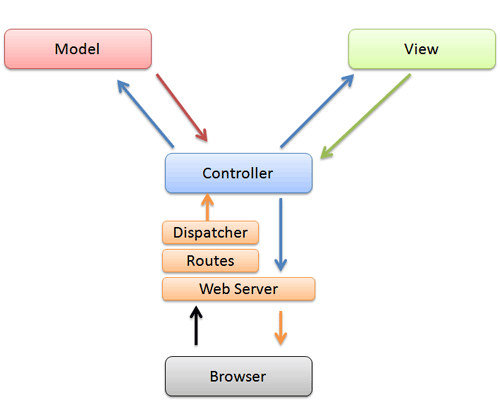
\includegraphics[scale=0.5]{src/mvc.png}
   \caption{\label{fig:mvc} MVC Architechture}
\end{figure}

Model-View-Controller is a very popular design pattern, for designing web
applications. Rails is an MVC framework, so following this architechture was
fairly simple.

In the Rails MVC, when the user makes a request for a page through his web
browser, the URL he ask for is routed to a particular method in a controller.
The job of the controller is to gather all the data from the model that
will have to be used in view. The view is then created with this data and is
sent back to the browser where the user can see the result. These interactions
can clearly be seen in figure~\ref{fig:mvc} on page~\pageref{fig:mvc}.

MVC is good way of creating a web application. It has a very clear design,
which allows for a clean separation of the different parts of the application,
and thus make the application very scalable. However MVC also has some
drawbacks. It sometimes unnecessarily complicates, things that should be simple.

\section{Architecture of the Database}

\begin{figure}[h]
   \centering
   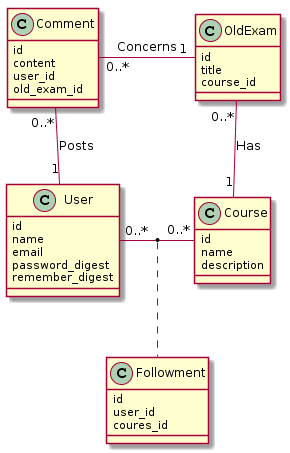
\includegraphics[scale=0.7]{src/digram.png}
   \caption{\label{fig:uml} Class Diagram of the Database}
\end{figure}


\section{Post Mortem}



\end{document}
